% !TEX program = xelatex
\documentclass[aspectratio=1610]{beamer}

\title{Učenje sa greškama}
\date{Jun 2026}
\author{Tanja Gavrić 1065/2025}

% Theme options — combine any of these in a single \usetheme call:
%   \usetheme[
%     pattern=triangle,
%     color=nudarkblue,
%     font=poppins,
%     numbering=progressbar,
%     sectionpage=on,
%     agendastyle=pattern
%   ]{wildcat}
%
% pattern: facet (default), facetrand, triangle, triangleiso, trianglemesh,
%          squares, circles, hexraise, hexrand, network, quilt, plain
% color: any named color (nu* colors are all available after theme loads).
%        All wcprimary shades are auto-generated. Omit to keep NU purple.
% font: noto (Noto Sans), poppins (Poppins+IBM Plex), nu (Campton+Akkurat),
%        installed (system fonts), or omit for default (Fira Sans — no files needed)
% numbering: fraction (default), number, progressbar, none
% sectionpage: on (default) or none
% agendastyle: plain (default) or pattern
% breadcrumb: on or none (default)
\usetheme[
    numbering=progressbar,
    sectionpage=on,
    agendastyle=pattern,
    breadcrumb=on
]{wildcat}

% You change the titlegraphic to whatever you want, or comment it out to remove it.
%\titlegraphic{
\includegraphics[scale=0.25]{logo-northwestern.pdf}}

\begin{document}

\begin{frame}
\titlepage
\end{frame}

\begin{frame}{Uvod}
    2016. godina - NIST objavljuje takmičenje za najbolje postkvantne kriptosisteme.
    \\ ~ \\
    8 godina kasnije, prvi standardizovan KEM algoritam je \textbf{ML-KEM}, zasnovan na ranijem algoritmu \textbf{CRYSTALS-Kyber}.
    \\ ~ \\
    \textbf{Cilj}: prikaz osnovne matematičke ideje iza ovog protokola.

    \begin{block}{Tok prezentacije}
        $
            \text{teški problemi na rešetkama}
            \quad \longrightarrow \quad
            \text{učenje sa greškama}
            \quad \longrightarrow \quad
            \text{Kyber}
        $
    \end{block}

\end{frame}

\begin{frame}[plain]
    \tableofcontents
\end{frame}

\section{Složenost problema}

\begin{frame}[fragile]

    Nije dovoljno reći: \emph{„Problem je težak.“}

    \begin{block}{Teorija složenosti}
        \textbf{NP-kompletni} problemi - najteži problemi klase NP.
    \end{block}

    \begin{palertblock}{Pažnja}
        \[
            \text{NP-kompletno} \neq \text{automatski dobro za kriptografiju}
        \]
    \end{palertblock}

    \begin{exampleblock}{Primjer}
        Merkle-Helman kriptosistem zasnovan na NP-kompletnom problemu ranca,
        može se razbiti tehnikama zasnovanim na LLL algoritmu.
    \end{exampleblock}

\end{frame}

\begin{frame}[fragile]

    \begin{block}{Problem}
        NP-kompletnost garantuje samo težinu \emph{najgoreg slučaja}, a nama je potrebna težina
        \emph{prosječnog slučaja}.
    \end{block}

    \begin{exampleblock}{Rješenje}
        Redukcija:

        \centering{
            \begin{array}{ccc}
                \text{najgori slučaj}
                & \Longrightarrow
                & \text{prosječan slučaj}
            \end{array}
        }
    \end{exampleblock}

    \only<2>{Problemi na rešetkama imaju ovakve redukcije!}
    \\ ~ \\

    \centering
    \begin{array}{ccc}
        \only<2>{\textcolor{nudarkgreen}{\text{problemi na rešetkama}}}
        & \only<2>{\Longrightarrow}
        &
        \only<2>{\textcolor{nudarkgreen}{\text{LWE}}}
    \end{array}

\end{frame}

\section{Učenje sa greškama, LWE}

\begin{frame}[fragile]{Primjer bez grešaka}
    \[
        \begin{aligned}
            2s_1+s_2 &= 7,\\
            s_1+3s_2 &= 11,\\
            3s_1+2s_2 &= 12.
        \end{aligned}
    \]

    Učimo skrivenu linearnu vezu:

    $s=(2,3)$.

\end{frame}

\begin{frame}[fragile]{Primjer sa greškama}

    \[
        \begin{aligned}
            2s_1+s_2 &= 7 \textcolor{red}{+1},\\
            s_1+3s_2 &= 11 \textcolor{red}{-1},\\
            3s_1+2s_2 &= 12 \textcolor{red}{+2}.
        \end{aligned}
    \]

    \begin{center}
        \Large
        Mala greška kvari jednostavnost početnog problema.
    \end{center}

\end{frame}

\begin{frame}[fragile]{Učenje sa greškama, LWE (Learning with errors)}

    Neka je $q$ prirodan, najčešće prost broj, i neka je $\mathbb{Z}_q = \mathbb{Z}/q\mathbb{Z}$ skup ostataka po modulu $q$.
    Neka su matrica $A \in \mathbb{Z}_q^{n \times m},$
    tajni vektor $s \in \mathbb{Z}_q^m$,
    i vektor greške $e \leftarrow D_{\mathbb{Z}^n,\sigma}$.

    \[
        \textcolor{blue}{b}
        =
        \textcolor{blue}{A}\cdot\textcolor{red}{s}
        +
        \textcolor{red}{e}
        \pmod q
    \]

    \[
        \textcolor{blue}{A,b} \text{ su poznati }
        \qquad
        \textcolor{red}{s,e} \text{ su nepoznati }
    \]

\end{frame}

\begin{frame}[fragile]{Geometrijska veza sa rešetkama}

    \[
        \mathcal{L} = \Lambda_q(\textcolor{nupurple}{A}^T) =
        \{x \in \mathbb{Z}^n \mid x \equiv \textcolor{nupurple}{A} \cdot z \pmod q,\ z \in \mathbb{Z}^m \}
    \]

    %\frametitle{Using Colors in Graphs}
    \begin{figure}
        \centering
        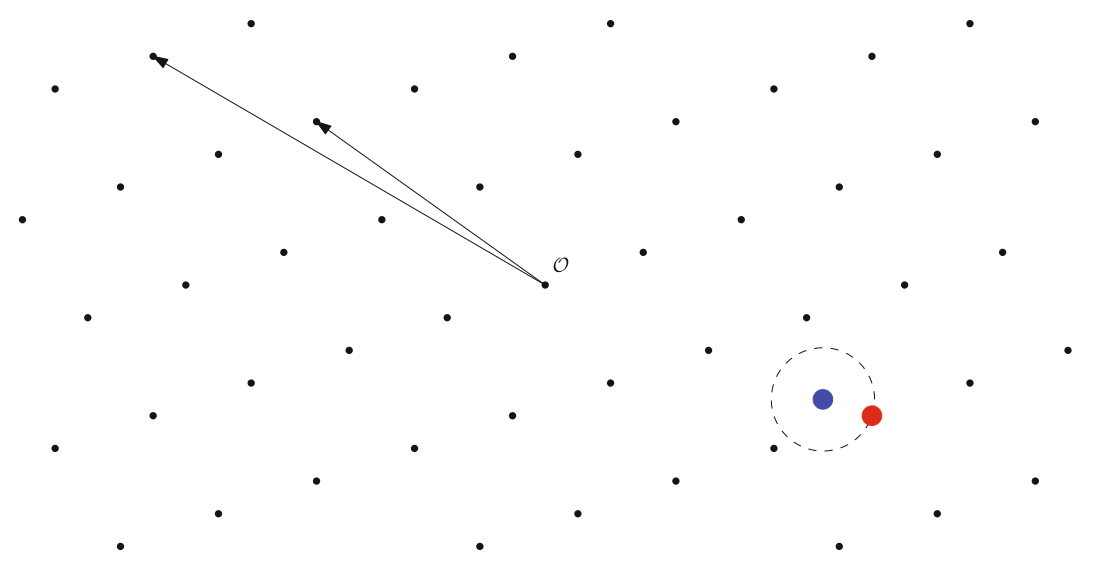
\includegraphics[width=0.62\textwidth]{./images/resetka.png}
        \label{fig:resetka}
    \end{figure}


    \[
        \textcolor{red}{A \cdot s} \in \mathcal{L},
        \qquad
        \textcolor{blue}{b} = \textcolor{red}{A \cdot s} + e,
        \qquad
        \textcolor{blue}{b} \text{ je blizu rešetke.}
    \]

\end{frame}

\begin{frame}[fragile]{Redukcija}

    Procenjujemo normu vektora $e$ kao $ \|e\| \leq \frac{2 \cdot \sigma \cdot \sqrt{m}}{\sqrt{2} \cdot \pi} $.

    Može se poistovijetiti sa $BDD_\alpha$ problemom, gde je
    $ \alpha = \frac{2\sigma\sqrt{m}}{\sqrt{2}\pi \lambda_1(\latt)} $.

    \begin{block}{Redukcija}
        \centering
        $BDD_\alpha$ \Longrightarrow LWE
    \end{block}

\end{frame}

\begin{frame}[fragile]{Protokol javnog ključa učenja sa greškama}
    \begin{columns}[T,onlytextwidth]
        \begin{column}{0.48\textwidth}
            \begin{block}{Generisanje ključa}
                $ \textcolor{red}{s} \in \mathbb{Z}_q^n $ \qquad
                $ \textcolor{blue}{a_i} \in \mathbb{Z}_q^n $ \qquad
                $ \textcolor{red}{e_i} \leftarrow D_{\mathbb{Z},\sigma} $

                $ \textcolor{blue}{b_i} = \textcolor{blue}{a_i} \cdot \textcolor{red}{s} - 2\cdot\textcolor{red}{e_i} \pmod q $
            \end{block}
        \end{column}

        \begin{column}{0.48\textwidth}
            \begin{block}{Enkripcija}
               % $ {\color{red}\iota_i} \in \{0,1\} $

                $ {\color{blue}c} = \sum_{i=1}^{m} {\color{red}\iota_i} {\color{blue}a_i} \pmod q $ \quad $ {\color{red}\iota_i} \in \{0,1\} $

                $ {\color{blue}d} = {\color{red}M} - \sum_{i=1}^{m} {\color{red}\iota_i} {\color{blue}b_i} \pmod q $
            \end{block}
        \end{column}

    \end{columns}

    \begin{block}{Dekripcija}
        \[
            \begin{aligned}
                {\color{blue}c} \cdot {\color{red}s} + {\color{blue}d} \pmod q
            &=
                \left(\sum_{i=1}^{m} {\color{red}\iota_i} {\color{blue}a_i}\right) \cdot {\color{red}s}
                + {\color{red}M}
                - \sum_{i=1}^{m} {\color{red}\iota_i} {\color{blue}b_i} \pmod q \\
                &=
                \sum_{i=1}^{m} {\color{red}\iota_i} ({\color{blue}a_i} \cdot {\color{red}s})
                + {\color{red}M}
                - \sum_{i=1}^{m} {\color{red}\iota_i} ({\color{blue}a_i} \cdot {\color{red}s} - 2{\color{red}e_i}) \pmod q \\
                &=
                    {\color{red}M} + 2\sum_{i=1}^{m} {\color{red}\iota_i} {\color{red}e_i} \pmod q = $ {\color{red}M} + \eta $
            \end{aligned}
        \]
    \end{block}

\end{frame}


\section{Učenje sa greškama u prstenu, Ring-LWE}

\begin{frame}[fragile]{Učenje sa greškama u prstenu}
    \begin{palertblock}{Nedostatak učenja sa greškama}
        Matrice izazivaju veliku memorijsku složenost. Dakle, LWE ima velike ključeve.
    \end{palertblock}

    \begin{exampleblock}{Rješenje - matrice postaju polinomi}
        \[
            b = A \cdot s+e
            \qquad \longrightarrow \qquad
            b = a\cdot s+e
        \]
    \end{exampleblock}

    Umjesto u $\mathbb{Z}_q^{n \times m}$, radićemo u prstenu polinoma $ R_q = (\mathbb{Z}/q\mathbb{Z})[X]/(F(X)) $.

\end{frame}


\begin{frame}[fragile]{Protokol javnog ključa učenja sa greškama u prstenu}
    \begin{columns}[T,onlytextwidth]
        \begin{column}{0.48\textwidth}
            \begin{block}{Generisanje ključa}
                $ \textcolor{red}{s,e} \leftarrow D_{R},\sigma $ \qquad
                $ \textcolor{blue}{a} \in R_q $

                $ {\color{blue}b} = {\color{blue}a} \cdot {\color{red}s} + p \cdot {\color{red}e} \pmod q $.
            \end{block}
        \end{column}

        \begin{column}{0.48\textwidth}
            \begin{block}{Enkripcija}
                $ {\color{red}e_0},{\color{red}e_1},{\color{red}e_2} \leftarrow D_{R,\sigma} \\
                {\color{blue}c_0} = {\color{blue}b} \cdot {\color{red}e_0} + p \cdot {\color{red}e_1} + {\color{red}M} \pmod q \\
                {\color{blue}c_1} = {\color{blue}a} \cdot {\color{red}e_0} + p \cdot {\color{red}e_2} \pmod q $
            \end{block}
        \end{column}

    \end{columns}

    \begin{block}{Dekripcija}
        \[
        \begin{aligned}
        {\color{blue}c_0} - {\color{blue}c_1} \cdot {\color{red}s}
        &=
        ({\color{blue}b} \cdot {\color{red}e_0} + p \cdot {\color{red}e_1} + {\color{red}M})
        -
        ({\color{blue}a} \cdot {\color{red}e_0} + p \cdot {\color{red}e_2})\cdot {\color{red}s} \pmod q \\
        &=
        (({\color{blue}a} \cdot {\color{red}s} + p \cdot {\color{red}e})\cdot {\color{red}e_0} + p \cdot {\color{red}e_1} + {\color{red}M})
        -
        ({\color{blue}a} \cdot {\color{red}e_0} \cdot {\color{red}s} + p \cdot {\color{red}e_2} \cdot {\color{red}s}) \pmod q \\
        &=
        p \cdot {\color{red}e} \cdot {\color{red}e_0} + p \cdot {\color{red}e_1} + {\color{red}M}
        -
        p \cdot {\color{red}e_2} \cdot {\color{red}s} \pmod q \\
        &=
        {\color{red}M} + p \cdot ({\color{red}e} \cdot {\color{red}e_0} + {\color{red}e_1} - {\color{red}
        e_2} \cdot {\color{red}s}) \pmod q = {\color{red}M} + p \cdot \eta
        \end{aligned}
        \]
    \end{block}

\end{frame}

\section{Kyber}

\subsection{Modulno učenje sa greškama}

\begin{frame}{Modulno učenje sa greškama}

    \begin{palertblock}{Nedostatak Ring-LWE pristupa}
        Za Ring-LWE postoje redukcije iz najgoreg u prosječan slučaj,
        ali se one odnose samo na probleme nad \emph{idealnim} rešetkama.
    \end{palertblock}

    \begin{exampleblock}{Ideja Module-LWE}
        Umjesto jednog polinoma, radimo sa $k$-strukim Dekartovim proizvodom prstena polinoma $R_q$:
        \[
            \mathbb{Z}_q^n
            \qquad \longrightarrow \qquad
            R_q^k
        \]
    \end{exampleblock}

    \[
        A \in R_q^{k \times k},
        \qquad
        s,e \in R_q^k,
        \qquad
        b = A \cdot s + e \pmod q.
    \]

    \begin{center}
        Module-LWE čuva efikasnost Ring-LWE pristupa, ali daje fleksibilniju strukturu.
    \end{center}

\end{frame}

\subsection{Module Lattices Key Encryption Mechnism, ML-KEM}

\begin{frame}{Kyber / ML-KEM u fazama}

    \[
        \text{Module-LWE}
        \longrightarrow
        \text{PKE šema}
        \longrightarrow
        \text{KEM protokol}
    \]

    \vspace{0.3cm}

    \begin{block}{1. Osnovna PKE (Public Key Encryption) šema}
        Na osnovu Module-LWE problema generiše se javni ključ:
        \[
            b = A \cdot s + e \pmod q
        \]
        gde je $A$ javna matrica nad $R_q^{k \times k}$, a $s$ i $e$ su mali tajni vektori polinoma.

        Enkripcija i dekripcija funkcionišu slično kao šeme LWE i Ring-LWE.
    \end{block}

    \begin{exampleblock}{2. KEM (Key Encapsulation Mechanism) protokol}
        Kyber primjenjuje „Fujisaki-Okamoto“ transformaciju
        \[
            \textsf{KeyGen}
            \rightarrow
            \textsf{Encaps}
            \rightarrow
            \textsf{Decaps}.
        \]
    \end{exampleblock}

\end{frame}


\begin{frame}{Primjena Kyber-a}
    \begin{itemize}
        \item \emph{CNSA 2.0} — Commercial National Security Algorithm Suite
        \item \emph{Google} — za podatke u tranzitu
        \item \emph{Signal} — zaštita poruka
        \item \emph{Apple} — iMesssage
        \item \emph{Amazon} — AWS Key Management Service
        \item \emph{IBM} — prototip uređaja za skladištenje podataka
    \end{itemize}
\end{frame}

\section{Pitanja}

\begin{frame}{Pitanja}
    \begin{enumerate}
        \item Kako izgleda protokol javnog ključa zasnovan na problemu učenja sa greškama?
        \item Objasniti geometrijsku intuiciju veze između problema dekodiranja na ograničenoj udaljenosti (BDD) i problema učenja sa greškama (LWE).
        \item Koje nedostatke osnovne šeme zasnovane na učenju sa greškama(LWE) ublažava njena varijanta učenja
        sa greškama u prstenu(Ring-LWE)?
    \end{enumerate}
\end{frame}


\end{document}
